\documentclass{article}
\usepackage[utf8]{inputenc}
\usepackage{amsmath,amssymb}
\usepackage{graphicx}
\usepackage[breaklinks=true]{hyperref}
\hypersetup{%
  colorlinks=true,% hyperlinks will be coloured
  %linkcolor=green,% hyperlink text will be green
  %linkbordercolor=red,% hyperlink border will be red
}
\DeclareMathOperator*{\argmax}{argmax} % thin space, limits underneath in displays
\DeclareMathOperator*{\argmin}{argmin} % thin space, limits underneath in displays
\sloppy 


\title{Modeling as a way of trying to be \\less surprised}
\author{Jesse Murray}
\date{}

\begin{document}

\maketitle

% Introduce probability with Physics
What does the word \emph{probability} mean? One could argue that given the laws of physics and the initial conditions, all events are deterministic, so there is no such thing as probability. While we may know the laws of physics, we do not know the initial conditions of all particles in the Universe. Therefore, we do not know all of the relevant information that determines whether an event occurs or not. Due to this lack of complete information, we reason about the world under uncertainty and we quantify our uncertainty by assigning probabilities to events. 

\begin{figure}
    \centering
    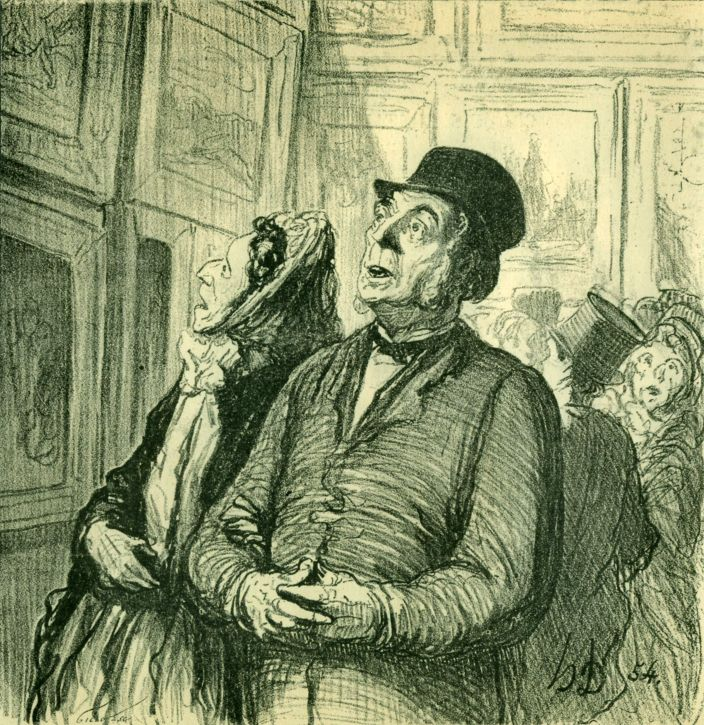
\includegraphics[scale=1.4]{images/surprise_painting.jpg}
    \caption{Sunday at the Museum, Honoré Daumier.}
    \label{fig:surprise_painting}
\end{figure}


\subsubsection*{Two interpretations of probability}
There are two broad interpretations of the probability $p \in (0, 1)$ of an event. (1) The \href{https://en.wikipedia.org/wiki/Frequentist_probability}{frequentist interpretation} considers probability to be the relative frequency of an event's occurrence as the situation in which the event could occur is repeated indefinitely. For example, if we consider flipping a weighted coin hundreds of times and observing it land heads about 42\% of the time, we could estimate from this frequency that the coin has probability $p=0.42$ of landing heads. The frequentist definition may be unwieldy however when we consider more unique, one-off situations, e.g., the 2024 US Presidential election. (2) The \href{https://en.wikipedia.org/wiki/Bayesian_probability}{Bayesian interpretation} is more suitable for such situations, as it considers probability to be one's degree of belief or opinion that an event will occur. That is, probability is defined as a final representation of one's state of knowledge about the occurrence of an event, based on a logical assessment of prior observations and evidence. One could imagine a Bayesian believing that if the future of the Universe were split into many equally possible branches, the event would occur in the fraction $p$ of these branches. 


\subsubsection*{Definition of Surprise}
Now let us define surprise. As you might expect, the term simply measures how surprised we are by the occurrence of an event. If an event with probability $p$ occurs, then our amount of `surprise' is $\log(1/p)$. This makes sense if we consider an event that has a 100\% probability of occurring. We should have 0 surprise when it occurs, and indeed $\log(1/1) = 0$. Likewise, if an event occurred that we mistakenly believed had probability $p = 0$ (let us imagine the calculus version of $p$ infinitely approaching 0). Then, our surprise is $\log(1/0) = \log(\infty) = \infty$. This is why you should never assign a probability of 0 to any event, because then if it occurs, you will either be infinitely surprised or undefined. 

%\newpage

\newcommand{\ptype}[1]{$p_{\mathrm{#1}}(\textbf{x})$}

%Explain KL Divergence with surprise
\subsubsection*{Kullback-Leibler divergence}
Surprise is closely related to the \href{https://en.wikipedia.org/wiki/Kullback\%E2\%80\%93Leibler_divergence}{Kullback-Leibler (KL) divergence}, which is a measure of how different two probability distributions are. To explain this, we must first explain the concept of expected surprise. Let $p_{\mathrm{true}}$ be the true probability distribution over observations $\textbf{x}\in\mathcal{X}$ such that \ptype{true} gives the true probability of observing of $\textbf{x}$. For our weighted coin example, $\textbf{x}$ $=$ the event that the coin lands heads. This event is an element of the set $\mathcal{X}$, which is the space of all possible events considered by the probability distribution (there are only two -- either the coin lands heads or tails). Suppose then that the coin actually lands heads with probability \ptype{true} $=$ 42.690\dots\%. (For the sake of simplicity, I'm intentionally conflating the event space with the domain of a random variable, and the realization of an event with the realization of a random variable.) Let $p_{\mathrm{model}}$ be our model probability distribution, which is our current guess for $p_{\mathrm{true}}$ (we guessed \ptype{model} = 42.0\%). 

For the uninitiated, $\mathbb{E}_{\textbf{x} \sim p_{\mathrm{distr}}} \bigr[ f(\textbf{x}) \bigr]$ is the \href{https://en.wikipedia.org/wiki/Expected_value}{expected value} of the function $f(\textbf{x})$ when the events $\textbf{x}\in\mathcal{X}$ occur (i.e. are \emph{distributed}) according to the probability distribution $p_{\mathrm{distr}}$. (Expected value and expectation are exactly the same concept as average or mean.)  If our function $f$ is surprise, then the average amount of surprise we experience by using our model is $\mathbb{E}_{\textbf{x} \sim p_{\mathrm{true}}} \bigr[ \log (1/p_{\mathrm{model}}(\textbf{x})) \bigr]$, because the data is distributed according to $p_{\mathrm{true}}$ and our function is $\log (1/p_{\mathrm{model}}(\textbf{x}))$. If instead of using an imperfect model, we know the true distribution $p_{\mathrm{true}}$, then our expected surprise is $\mathbb{E}_{\textbf{x} \sim p_{\mathrm{true}}} \bigr[ \log (1/p_{\mathrm{true}}(\textbf{x})) \bigr]$. 

KL-Divergence is typically understood as a measure of how one probability distribution is different from a second, reference probability distribution. When we let those two probability distributions be $p_{\mathrm{true}}$ and $p_{\mathrm{model}}$, the equation for KL-Divergence is:
\begin{equation*}
D_{KL}(p_{\mathrm{true}} || p_{\mathrm{model}}) =  \mathbb{E}_{\textbf{x} \sim p_{\mathrm{true}}} \bigr[ \log (1/p_{\mathrm{model}}(\textbf{x})) \bigr] \, - \, \mathbb{E}_{\textbf{x} \sim p_{\mathrm{true}}} \bigr[ \log (1/p_{\mathrm{true}}(\textbf{x})) \bigr] \ .
\end{equation*}
We can see that the KL-divergence to $p_{\mathrm{true}}$ from $p_{\mathrm{model}}$ is the expected excess surprise from using our imperfect model $p_{\mathrm{model}}$ rather than the ground truth $p_{\mathrm{true}}$. That is, the KL-divergence measures the \emph{extra} amount of surprise we experience on average when the actual data is distributed according to $p_{\mathrm{true}}$ but we are instead working with $p_{\mathrm{model}}$. It's the price we pay -- in terms of being surprised -- for having the wrong model. It can be shown with \href{https://en.wikipedia.org/wiki/Jensen\%27s_inequality}{Jensen's inequality} that the KL-divergence is always positive, except when $p_{\mathrm{model}} = p_{\mathrm{true}}$, when it is clearly equal to zero. This means that we are always more surprised on average when we are working with the wrong probabilities than when we work with the correct probabilities, which makes intuitive sense. 

\subsubsection*{Model selection with KL-divergence minimization}
KL-divergence is important in statistics and machine learning because we choose our model by minimizing the KL-divergence. We can now understand this process of model selection as minimizing how surprised we are on average by using our model. Minimizing KL-divergence is also called minimizing the cross-entropy (average surprise is also called \href{https://en.wikipedia.org/wiki/Entropy_(information_theory)}{entropy}), and we are taking the \emph{cross} (i.e. the difference through subtraction) between our model's entropy $\mathbb{E}_{\textbf{x} \sim p_{\mathrm{true}}} \bigr[ \log (1/p_{\mathrm{model}}(\textbf{x})) \bigr]$ and the irreducible ground truth entropy $\mathbb{E}_{\textbf{x} \sim p_{\mathrm{true}}} \bigr[ \log (1/p_{\mathrm{true}}(\textbf{x})) \bigr]$. Minimizing the KL-divergence is also equivalent to finding the \href{https://en.wikipedia.org/wiki/Bayes_estimator}{Bayes estimator} when our cost function is surprise. One could imagine that we are pained by surprise and therefore want to expect as little of the emotion as possible, however we have no bias towards the kind of surprise we experience. That is, we do not have a preference for or against being surprised by making a false positive or a false negative (for classification tasks), or by overestimating or underestimating (for regression tasks). 


This concept of surprise tends to favour the Bayesian definition of probability. Surprise can be viewed as the emotion one experiences when one's beliefs $p_{\mathrm{model}}$ do not match reality $p_{\mathrm{true}}$. We see however that even when our beliefs are correct ($p_{\mathrm{model}} = p_{\mathrm{true}}$), we still experience an irreducible amount of surprise on average (i.e. entropy) given by $\mathbb{E}_{\textbf{x} \sim p_{\mathrm{true}}} \bigr[ \log (1/p_{\mathrm{true}}(\textbf{x})) \bigr]$, we cannot get any less surprised than this. The irreducibility of this surprise begs the question of what we mean by $p_{\mathrm{true}}$. We said earlier that if we knew everything about the Universe, then every observed event has probability 1. That is, the omniscient observer is never surprised. We consider the existence of $p_{\mathrm{true}}$ only because we imagine there is some level of irreducible uncertainty in the universe. 


For example, suppose we want to predict some target $y$ (e.g. the height of a child) based on known observations $\textbf{x}$ (e.g. the heights of the child's parents). Then $p(y|\textbf{x})$ gives the \href{https://en.wikipedia.org/wiki/Conditional_probability}{conditional probability} of the target $y$ based on the observations $\textbf{x}$. This mapping from our observations $\textbf{x}$ to our target $y$ may be inherently stochastic. That is, there may be some completely unpredictable biological randomness in the determination of height. Or, perhaps $y$ \emph{is} deterministic but depends on other variables not included in $\textbf{x}$, which we therefore do not observe, e.g., the specific alleles of the parents and the diet of the child. Whether the system is either inherently stochastic or we do not have all the necessary information, the ground truth  $p_{\mathrm{true}}(y|\textbf{x})$ is in either case entropic (i.e. surprising). The lowest error we could possibly hope to obtain by our model, the error we would incur if we were an oracle making predictions from this `true' distribution, is known as the \href{https://en.wikipedia.org/wiki/Bayes_error_rate}{Bayes error rate}. That is, with surprise as our cost function, the Bayes error rate is the irreducible average surprise given by $\mathbb{E}_{\textbf{x} \sim p_{\mathrm{true}}} \bigr[ \log (1/p_{\mathrm{true}}(\textbf{x})) \bigr]$.

\subsubsection*{KL-divergence minimization is maximum likelihood estimation}
If we were to try to minimize the KL-divergence of our model in the way just described, we would need access to $p_{\mathrm{true}}$. Unfortunately, this is almost never the case (if we knew $p_{\mathrm{true}}$, then there would be no need to build $p_{\mathrm{model}}$). As an approximation to $p_{\mathrm{true}}$, we use $\hat{p}_{\mathrm{data}}$, which is simply the dataset, i.e., the empirical distribution of the observations. It consists of paired observations $\textbf{x}$ and $y$. This is where the term \emph{training} comes from in machine learning, as we typically split the dataset randomly into a set for \emph{training} the model (showing it observations of $\textbf{x}$ paired with $y$) and a separate set for \emph{testing} the performance of model (showing it only $\textbf{x}$ and asking it to predict $y$). We hope that the model, which is like a `machine', \emph{learns} effectively from the training set, hence we call it machine learning. Admittedly, the terminology is a bit pretentious. By using this method, we are hoping that the empirical distribution of the data $\hat{p}_{\mathrm{data}}$ matches $p_{\mathrm{true}}$, which is more likely to occur in large diverse datasets that converge with fidelity to the population distribution of possible events. We also hope that there is sufficient dependency between our target $y$ and the information provided within each observation $\textbf{x}$ such that our target $y$ \emph{could} in theory be predicted from $\textbf{x}$.

As a way of selecting the optimal $p_{\mathrm{model}}$ (the one that minimizes the KL-divergence) it is often most convenient to utilize a parametric family of probability distributions $p_{\mathrm{model}}(\textbf{x} , \boldsymbol{\theta})$, which defines a space of possible models indexed by the parameter $\boldsymbol{\theta}$ (note that $\boldsymbol{\theta}$ can be an array of multiple constituent parameters). We then search for the optimal model within this space of models by searching for the best parameter $\boldsymbol{\theta}$. By optimal model, we mean the one that gets as close as possible to the elusive $p_{\mathrm{true}}$. The KL-divergence minimization is therefore performed by adjusting the parameter $\boldsymbol{\theta}$. In practice, we must use $\hat{p}_{\mathrm{data}}$ in place of $p_{\mathrm{true}}$, in which case our KL-divergence is
\begin{equation*}
D_{KL}(p_{\mathrm{true}} || p_{\mathrm{model}}) =    \mathbb{E}_{\textbf{x} \sim \hat{p}_{\mathrm{data}}} \bigr[ \log (1/p_{\mathrm{model}}(\textbf{x}; \boldsymbol{\theta})) \bigr] \, - \, \mathbb{E}_{\textbf{x} \sim \hat{p}_{\mathrm{data}}} \bigr[ \log (1/\hat{p}_{\mathrm{data}}(\textbf{x})) \bigr] 
\end{equation*}
We can neglect the term on the right in the minimization procedure because it is simply a function of the data, not of $\boldsymbol{\theta}$. We therefore simply need to find the parameter $\boldsymbol{\theta}$ that minimizes 
\begin{equation*}
\mathbb{E}_{\textbf{x} \sim \hat{p}_{\mathrm{data}}} \bigr[ \log (1/p_{\mathrm{model}}(\textbf{x}; \boldsymbol{\theta})) \bigr]
\end{equation*}


It might surprise you that this minimization is identical to \href{https://en.wikipedia.org/wiki/Maximum_likelihood_estimation}{maximum likelihood estimation (MLE)}. We can see this connection if we look at the definition of the maximum likelihood estimator for $\boldsymbol{\theta}$ (for $n$ observations $\textbf{x}^{(i)}$ in the data):
\begin{equation*}
% \boldsymbol{\theta}_{\mathrm{ML}} = \argmax_{\boldsymbol{\theta}} \sum_{i=1}^n \log( p_{\mathrm{model}}(\textbf{x}^{(i)}; \boldsymbol{\theta})) \ ,
\begin{aligned}
\boldsymbol{\theta}_{\mathrm{MLE}} {} &=
\argmax_{\boldsymbol{\theta}}   \, p_{\mathrm{model}}(\text{data}; \boldsymbol{\theta}) \\ &=
\argmax_{\boldsymbol{\theta}}  \, \log(\prod_{i=1}^n p_{\mathrm{model}}(\textbf{x}^{(i)}; \boldsymbol{\theta})) \\ &=
\argmax_{\boldsymbol{\theta}} \, \sum_{i=1}^n \log( p_{\mathrm{model}}(\textbf{x}^{(i)}; \boldsymbol{\theta})) \\ &= \argmax_{\boldsymbol{\theta}} \, \mathbb{E}_{\textbf{x} \sim \hat{p}_{\mathrm{data}}} \bigr[ \log( p_{\mathrm{model}}(\textbf{x};  \boldsymbol{\theta})) \bigr] \\ &= \argmin_{\boldsymbol{\theta}} \, \mathbb{E}_{\textbf{x} \sim \hat{p}_{\mathrm{data}}} \bigr[ \log( 1/p_{\mathrm{model}}(\textbf{x};  \boldsymbol{\theta})) \bigr] \ .
\end{aligned}
\end{equation*}
We typically think of MLE as picking the parameter $\boldsymbol{\theta}$ that maximizes the probability of observing the dataset, under the assumption that the data points are approximately independent and identically distributed according to $p_{\mathrm{true}}$ and $p_{\mathrm{true}}$ is within the parametric family $p_{\mathrm{model}}(\textbf{x} , \boldsymbol{\theta})$. Now, we see that this method is equivalent to minimizing the expected surprise, under this same assumption.  

\subsubsection*{Linear regression is Gaussian surprise minimization}
If you've ever used linear regression, you've performed MLE. Linear regression makes predictions with a linear combination of observed features $\textbf{x}$, weighted by $\boldsymbol{\theta}$, and penalizes the sum of the squared errors between the predictions and the observed data. In this way, the model obtains the hyperplane of best fit in the space $\mathcal{X} \cup \mathbb{R}$ (where $\textbf{x}\in\mathcal{X}$ and $y\in \mathbb{R}$). Penalizing the squared error is equivalent to assuming a Gaussian parametric model $p_{\mathrm{model}}(y | \textbf{x} , \boldsymbol{\theta}) = \mathcal{N}(\boldsymbol{\theta}^T \textbf{x}, 1)$ in which the data is assumed to be normally distributed (with irrelevant variance for making predictions) about the prediction $\boldsymbol{\theta}^T \textbf{x}$. The equivalency between the squared error cost and the Gaussian parametric family arises simply because the \href{https://en.wikipedia.org/wiki/Normal_distribution}{Gaussian probability density function} actually contains the squared difference between the prediction $\boldsymbol{\theta}^T \textbf{x}$ and the observed target $y$: $(y \, - \, \boldsymbol{\theta}^T\textbf{x})^2$ in an exponential and that exponential is stripped away when the $\log$ is applied in the $\boldsymbol{\theta}_{\mathrm{MLE}}$ summation (as shown above). Likewise, the product of the joint probability of independent and identically distributed observations becomes the sum of the terms in the exponential (the squared error), as the $\log$ operation turns a product $\Pi$ to a sum $\Sigma$ (also as shown above). This is why MLE with the Gaussian parametric family is equivalent to minimizing the sum of the squared errors, i.e., the method of least squares. Therefore, we see that using the squared error as the cost function is identical to using surprise as the cost function and assuming the data is Gaussian distributed (both approaches have the same Bayes estimator). 

\subsubsection*{Surprise is also information content}
It should also be noted that surprise is also known as \href{https://en.wikipedia.org/wiki/Information_content}{information content} (or Shannon information). This makes sense when we consider the obvious fact that learning that an unlikely event has occurred is more informative than learning that a likely event has occurred. In the extreme case, when we learn that an event occurred that we believed had a 100\% chance of occurring, we are clearly provided with with no new information. We often use base-2 for the logarithm in $\log(1/p)$, so that the amount of information provided by an event can be measured in bits (an event that has probability $p=1/2$ provides one bit of information when it occurs). In this view, the entropy of a probability distribution tells us the average amount of information provided by an event drawn from that distribution. Equivalently, the entropy gives us the number of bits needed on average to encode events drawn from that distribution, e.g., if we were communicating the outcome of the events over a communication channel and wanted to use as few bits as possible. 

\subsubsection*{Surprise in everyday life}
%Break the fourth wall
This is getting a bit rambly. There's more I want to say about surprise so I should continue this in a second blog post. The main reason I thought surprise was interesting is that I think it is a connection between statistics and the human emotional experience. It is the feeling of surprise that repeatedly teaches us the hard lesson that the world indeed is probabilistic, not deterministic, and that we cannot predict the future perfectly. By understanding ideas of probability and statistics in terms of surprise, we can see these same ideas from the same intuitive perspective we use for our every-day understanding of the world and hopefully then gain a deeper intuitive understanding of statistics. 

Instead of thinking of modeling as maximizing likelihood, whatever that means, we can think of modeling as a way of trying to be less surprised by events. We make our model of the world under a surprise-minimization framework, which tends to be how we go through our lives anyways. Perhaps this is part of our brains' vestigial survival mechanism. Our \href{https://en.wikipedia.org/wiki/Ecological_niche}{ecological niche} was having sophisticated brains that could form a high-fidelity model of the complex world around us and act on those models, finding ingenious and resourceful paths to evolutionary success. Even if our model was technically wrong, as long as it was useful, it was good. This goes with the well-known saying in statistics: \href{https://en.wikipedia.org/wiki/All_models_are_wrong}{All models are wrong, but some are useful}. Much of our model of the world exists within intuition and common sense: that \href{https://en.wikipedia.org/wiki/Unconscious_mind}{ineffable knowledge-base} that shapes our actions through some automatic, neigh latent mechanism. This model can be updated by the emotion of surprise and its associated valence, depending on the event that elicits it. On the other hand, when someone makes the sly comment in response to some piece of news `I'm not surprised,' often what they are really saying is that their mental model of the world had placed a relatively high degree of belief or probability in the event possibly occurring and they may even feel some pride in the fidelity of their mental model. 

There is a tendency among humans to perceive past events as having been more predictable than they actually were. This is known as \href{https://en.wikipedia.org/wiki/Hindsight_bias}{hindsight bias}. Perhaps we have this bias because surprise promotes a sense-making process in which we change our model of the world \cite{Mller2007}. Under our new updated model of the world, the event is more likely and we mistakenly misremember that we held this new model of the world all along. This might also explain why hindsight bias has been found to be more likely to occur when the outcome of an event is negative rather than positive \cite{Schkade1991}. We are more sensitive to negative events and our model of the world is updated more in response to the surprise of a negative event. That is, in our belief and expectation-forming process, we do not perform simple maximum likelihood estimation, because we change our model more in response to negative events than in response to positive events. None of us likes to be surprised by negative events, we do not like \href{https://en.wikipedia.org/wiki/Black_swan_theory}{black swans}. However being surprised by positive events can also be disorienting as it makes us realize that we had the wrong model of the world. We are confronted with the missed opportunities by having an overly pessimistic or conservative outlook. Now we can see the inherent cost function of our inner model: We penalize surprise, especially of negative events. Quoting the English journalist Walter Bagehot: ``One of the greatest pains to human nature is the pain of a new idea."

Since the surprise of an event is equivalent to the amount of information provided by it, we should be unsurprised (no pun intended) that modern information-providing outlets, that cater to the demands of our anachronistic brains, i.e. the news and media, tend to publicize unlikely events. Furthermore, to best update our Bayesian belief systems (models) about the world, we would expect these outlets to publicize the kinds of events that us humans are most sensitive to: negative events. Unsurprisingly as well, there is substantial research to show that the news tends to be negative, explaining the adage in media ``if it bleeds, it leads" \cite{Soroka2019}. As you read this now, please open up your favorite news website of choice, and I will bet you that within the top stories, there will be one about an event that is both relatively unlikely \emph{and} negative. If I am wrong then please send me a contemporaneous screenshot along with your bank details and I will transfer you £0.42. I should note that I got some of the ideas in this post from Joseph Blitzstein's \href{https://drive.google.com/file/d/1VmkAAGOYCTORq1wxSQqy255qLJjTNvBI/view}{Probability textbook} \cite{Blitzstein2014} and Ian Goodfellow's \href{https://www.deeplearningbook.org/}{Deep Learning textbook} \cite{Goodfellow2016}. I highly recommend giving both books a read.

\newpage

\bibliographystyle{unsrt}
\bibliography{surprise}

\end{document}

